\documentclass[11pt, a4paper, twoside]{article}

% Versión 1.er cuat 2021 Víctor Bettachini < vbettachini@unlam.edu.ar >

\usepackage[T1]{fontenc}
\usepackage[utf8]{inputenc}

% \usepackage[spanish, es-tabla]{babel}
\def\spanishoptions{argentina} % Was macht dass?
% \usepackage{babelbib}
% \selectbiblanguage{spanish}
% \addto\shorthandsspanish{\spanishdeactivate{~<>}}

\usepackage{graphicx}
\graphicspath{{./figuras/}{../LaTeX/}{../figurasLaTeX/}}
% \usepackage{float}

\usepackage[arrowdel]{physics}
\newcommand{\pvec}[1]{\vec{#1}\mkern2mu\vphantom{#1}}
% \usepackage{units}
\usepackage[separate-uncertainty= true, multi-part-units= single, range-units= single, range-phrase= {~a~}, locale= FR]{siunitx}
\usepackage{isotope} % $\isotope[A][Z]{X}\to\isotope[A-4][Z-2]{Y}+\isotope[4][2]{\alpha}

\usepackage{tasks}
\usepackage[inline]{enumitem}
% \usepackage{enumerate}

\usepackage{hyperref}

% \usepackage{amsmath}
% \usepackage{amstext}
% \usepackage{amssymb}

\usepackage{tikz}
\usepackage{tikz-3dplot}
\usepackage{tikz-dimline}
\usetikzlibrary{calc}
% \usetikzlibrary{math}
\usetikzlibrary{arrows.meta}
\usetikzlibrary{snakes}
\usetikzlibrary{decorations}
\usetikzlibrary{decorations.pathmorphing}
\usetikzlibrary{patterns}

\usepackage[hmargin=1cm,vmargin=3cm, top= 0.75cm,nohead]{geometry}

\usepackage{lastpage}
\usepackage{fancyhdr}
\pagestyle{fancyplain}
\fancyhf{}
\setlength\headheight{28.7pt} 
\fancyhead[LE, LO]{\textbf{Computational Analytical Mechanics} }
% \fancyhead[LE, LO]{\textbf{Mecánica General} }
\fancyhead[RE, RO]{\href{https://ingenieria.unlam.edu.ar/}{$\vcenter{\hbox{
\includegraphics[height=1cm]{../../../../figurasLaTeX/ambos.pdf}}}$}}  %edg fix path
\fancyfoot{\href{https://creativecommons.org/licenses/by-nc-sa/4.0/deed.es_ES}{$\vcenter{\hbox{
\includegraphics[height=0.4cm]{../../../../figurasLaTeX/by-nc-sa_80x15.pdf}}}$} \href{https://ingenieria.unlam.edu.ar/}{DIIT - UNLaM}}  %edg fix path
\fancyfoot[C]{ {\tiny Updated on \today} }
\fancyfoot[RO, LE]{Pág. \thepage/\pageref{LastPage}}
\renewcommand{\headrulewidth}{0pt}
\renewcommand{\footrulewidth}{0pt}



\begin{document}

\begin{center}
  \textsc{\large Generalized coordinates | Constraints | Kinetic and potential energies}
\end{center}
\noindent
Exercises marked with (*) have extra difficulty, don't hesitate to ask for help.

\begin{enumerate}

\item
	\begin{minipage}[t][5cm]{0.7\textwidth}
		\textbf{Pendulum with free point of support} [Landau \S5 ex. 2]\\
		Particle of mass $m_2$ is hanging from a rigid bar of length $\ell$ and negligible mass. On the other end there is a device of mass $m_1$ linked to a horizontal bar, and it's free to move horizontally along the $x$ axis. The device allows the hanging bar to span any angle $\varphi$ respect to the vertical axis. 
		\begin{enumerate}
			\item Write expressions for kinetic energy, $T$ and potential, $V$, as functions of the generalized coordinates suggested by the figure.
			\item Verify that if you fix the position of mass $m_1$ you recover the expressions of $T$ and $V$ of an ideal pendulum.
		\end{enumerate}
	\end{minipage}
	\begin{minipage}[c][1cm][t]{0.3\textwidth}
		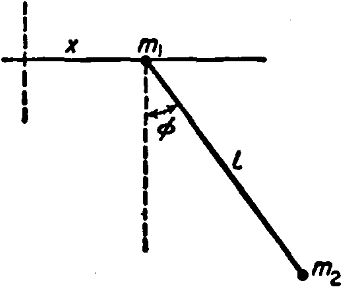
\includegraphics[width=0.75\textwidth]{figures/landauS52_fig2.png}
	\end{minipage}



\item
	\begin{minipage}[t][4cm]{0.7\textwidth}
		\textbf{Coplanar double pendulum} [Landau \S5 ex. 1]\\
		A ridig bar of lentgh $\ell_1$ of negligible mass has a particle of mass $m_1$ attached to one end. There is a second bar of negligible mass hanging from the first one, of length $\ell_2$, with a particle of mass $m_2$ attached to the other end too.
		\begin{enumerate}
			\item Write expressions for kinetic energy, $T$ and potential, $V$, as functions of the generalized coordinates suggested by the figure.
			\item Verify that you recover the expressions of $T$ and $V$ of an ideal pendulum if you set $m_1=0$, $\varphi_1 = \varphi_2 = \varphi$ and  $\ell_1 = \ell_2 = \frac{\ell}{2}$.
		\end{enumerate}
	\end{minipage}
	\begin{minipage}[c][0.5cm][t]{0.3\textwidth}
		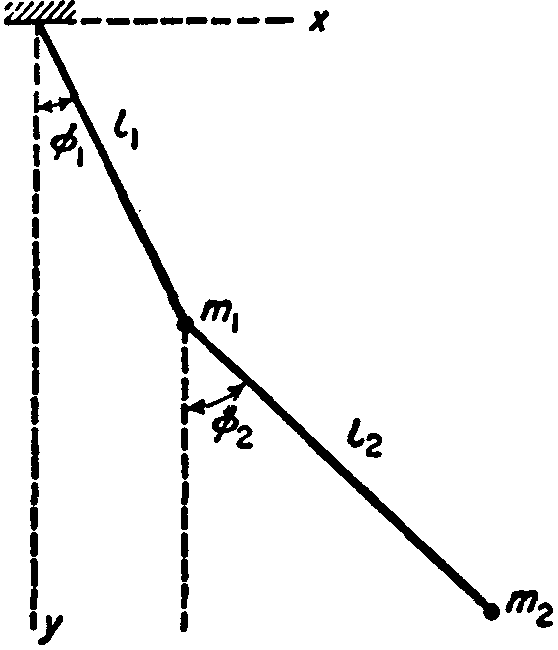
\includegraphics[width=0.75\textwidth]{figures/landauS52_fig1.png}
	\end{minipage}



\item
	\begin{minipage}[t][7.1cm]{0.5\textwidth}
		(*) \textbf{Pendulum with rotating point of support} [Marion (e) ex. 7.5] [Landau \S5 ex. 3]\\
		A particle of mass $m$ is attached to the end of a rigid bar of length $b$. The point of support is linked to a vertical circle of radius $a$ and it rotates with constant frequency $\omega$. It is assumed that all positions lie in the same plane and the mass of the bar is negligible. Calculate the kinetic energy, $T$, and potential $V$, of the particle of mass $m$.
	\end{minipage}
	\begin{minipage}[c][3cm][t]{0.5\textwidth}
		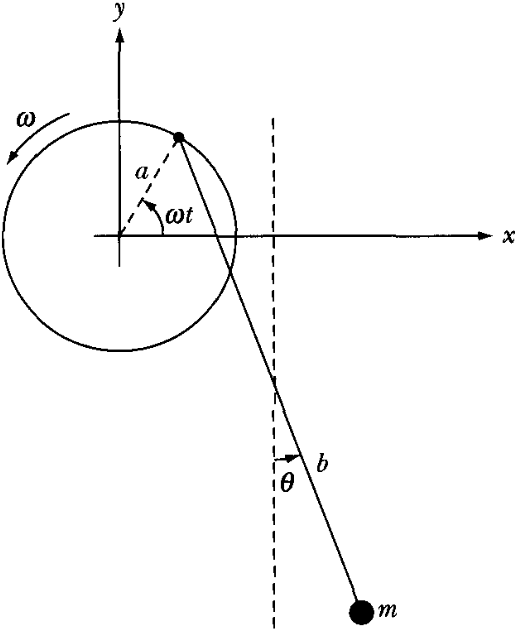
\includegraphics[width=0.75\textwidth]{figures/marion_fig7_3.png}
	\end{minipage}



\item
	\begin{minipage}[t][4.5cm]{0.65\textwidth}
		(*) \textbf{Coupled weights rotating about a vertical axis} [Landau \S5 ex. 4]\\
		Particle with mass $m_2$ moves on a vertical axis and the whole system rotates about this axis with a constant angular velocity $\Omega$. This particle is linked to two particles of mass $m_1$ through bars of length $a$ and negligible mass, and at the same time these particles are linked to the fixed point $A$ trough identical bars, forming the variable angle $\theta$ respect to the vertical axis.
		Calculate the kinetic energy of each of the three particles and find a compact expression of the kinetic energy of the whole system.
	\end{minipage}
	\begin{minipage}[c][1cm][t]{0.35\textwidth}
		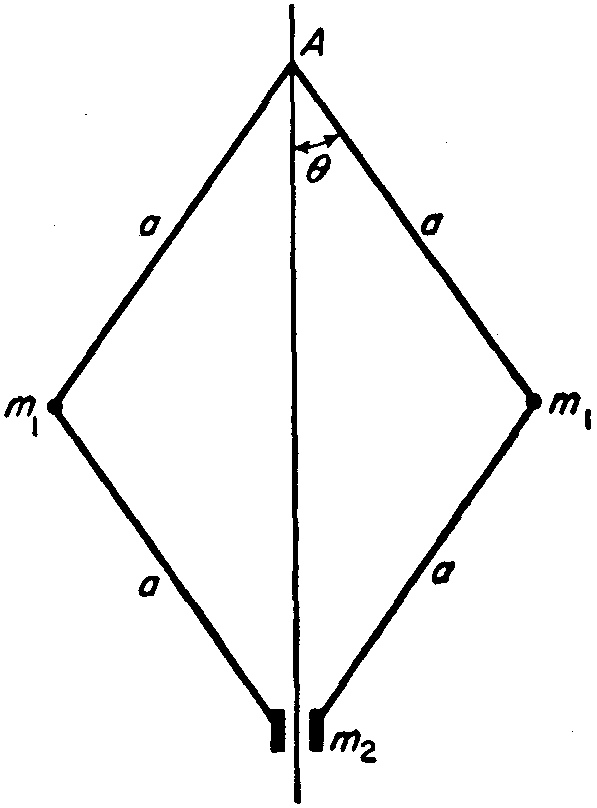
\includegraphics[width=0.75\textwidth]{figures/landauS52_fig4.png}
	\end{minipage}


\end{enumerate}
\end{document}
